\documentclass[journal,twoside]{IEEEtran}
\usepackage{amsmath,amssymb,amsfonts,amsthm}
\usepackage{booktabs}
\usepackage{graphicx}
\usepackage{cite}
\usepackage{array}
\usepackage{multirow}
\usepackage{hyperref}

\emergencystretch=1.5em
\allowdisplaybreaks[2]

\newtheorem{theorem}{Theorem}
\newtheorem{proposition}{Proposition}
\newtheorem{lemma}{Lemma}
\newtheorem{corollary}{Corollary}
\newtheorem{remark}{Remark}

\begin{document}
% AUTO-GENERATED BY src/export_metrics.py — DO NOT EDIT MANUALLY
\providecommand{\NumCaseStudies}{seven}
\renewcommand{\NumCaseStudies}{seven}
\providecommand{\MaxTVEProposed}{0.18\%}
\renewcommand{\MaxTVEProposed}{0.18\%}
\providecommand{\LatencyThirtyRange}{0.030\text{--}0.362\text{~ms}}
\renewcommand{\LatencyThirtyRange}{0.030\text{--}0.362\text{~ms}}
\providecommand{\LatencyOneEighteenRange}{0.047\text{--}5.865\text{~ms}}
\renewcommand{\LatencyOneEighteenRange}{0.047\text{--}5.865\text{~ms}}
\providecommand{\BlindSpotMs}{80\text{~ms}}
\renewcommand{\BlindSpotMs}{80\text{~ms}}


\title{Provably Resilient Synchrophasor State Estimation Under Coordinated Majority GPS Spoofing, Load Transients, and Substation Cyber-Physical Attacks}

\author{Mohd~Aarish~Shaheen and S.~A.~Soman%
\thanks{M.~A.~Shaheen is with the Department of Electrical Engineering, University of Kashmir (UoK), Srinagar, and the Indian Institute of Technology Bombay (IITB), Mumbai (e-mail: aarishshaheen@uok.edu.in).}%
\thanks{S.~A.~Soman is with the Department of Electrical Engineering, Indian Institute of Technology Bombay (IITB), Mumbai.}}

\maketitle

\begin{abstract}
Phasor Measurement Unit (PMU) state estimation executes at millisecond granularity in modern Wide-Area Monitoring, Protection, and Control (WAMPAC) centers. Because PMUs derive their phase angle reference from civilian Global Positioning System (GPS) 1-Pulse-Per-Second (1-PPS) timing strobes, they are acutely vulnerable to GPS Spoofing Attacks (GSAs). Recent hybrid architectures---most notably Badugu \emph{et al.} (2026)---achieve spoofing invariance by switching from complex Linear State Estimation (LSE) to a scalar Nonlinear Least Squares (NLS) solver triggered by a subspace Principal Angle (PA) test, recovering the Coordinated Universal Time (UTC) reference frame via one-dimensional (1D) DBSCAN clustering. This paper proves that such memoryless scalar-clustering architectures exhibit four structural failure modes: (i) an 80~ms (4-cycle) protection blind spot during persistence counter accumulation; (ii) reference-frame hijacking and chordal error amplification whenever $\ge 50\%$ of installed PMUs undergo a coordinated spoofing attack; (iii) zero statistical breakdown under simultaneous False Data Injection Attacks (FDIAs) or Analog-to-Digital Converter (ADC) channel corruptions; and (iv) $\mathcal{O}(m N_b^2)$ dense Jacobian and $\mathcal{O}(|\mathcal{P}|^2)$ spatial clustering overhead. To overcome these limitations, we formulate a Zero-Allocation, Fused Multi-Dimensional Robust Dynamic State Estimation (DSE) architecture. By integrating a sparse $\mathcal{O}(\mathrm{nnz}(R))$ Principal Angle screen, an $\mathcal{O}(m)$ 4-node graph-accumulated Huber M-estimator with in-place column-active sparse Symmetric Positive-Definite (SPD) Cholesky factorization, a 6-Dimensional Physical-Invariance Feature Manifold anchored to Center-of-Inertia (COI) swing dynamics, and an $\mathcal{O}(|\mathcal{P}|\log|\mathcal{P}|)$ order-statistic sort-clustering kernel, our estimator guarantees immunity even under $70\%$ coordinated majority spoofing coinciding with sudden $+18\%$ load steps and simultaneous FDIA/ADC faults. Validated on canonical MATPOWER IEEE 30-bus (13~PMUs) and IEEE 118-bus (54~PMUs) networks across seven comprehensive case studies, the proposed estimator maintains $\le \MaxTVEThirty$ Maximum Total Vector Error (TVE) across all attack regimes while executing in $\MinTimeThirty\text{--}\MaxTimeThirty\text{ ms}$ on IEEE 30-bus and $\MinTimeOneEighteen\text{--}\MaxTimeOneEighteen\text{ ms}$ on IEEE 118-bus---well within the 20~ms IEEE C37.118.1 real-time window.
\end{abstract}

\begin{IEEEkeywords}
Cyber-physical power systems, dynamic state estimation, false data injection attack, GPS spoofing, Huber M-estimation, numerical linear algebra, phasor measurement unit, principal angle, sparse Cholesky factorization.
\end{IEEEkeywords}

\section*{Nomenclature}
\addcontentsline{toc}{section}{Nomenclature}
\begin{IEEEdescription}[\IEEEusemathlabelsep\IEEEsetlabelwidth{$\Delta\theta_{k,t}^{\mathrm{phys,rel}}$}]
\item[$N_b, N_l$] Number of system buses and transmission branches.
\item[$\mathcal{P}, N_p$] Set and cardinality of PMU-instrumented buses ($N_p = \vert{}\mathcal{P}\vert{}$).
\item[$m, m_s$] Number of complex phasor channels and scalar measurements ($m_s = N_p + 2N_i$).
\item[$v, \hat{v}^{\mathrm{LSE}}$] True and complex WLS estimated nodal voltage vectors ($\in \mathbb{C}^{N_b}$).
\item[$z^{\mathrm{act}}, z^{\mathrm{spf}}$] Unattacked and GPS-spoofed complex PMU measurement vectors ($\in \mathbb{C}^m$).
\item[$H, \tilde{H}$] Complex measurement Jacobian and whitened matrix ($\tilde{H} = W^{-1/2}H \in \mathbb{C}^{m \times N_b}$).
\item[$W, R$] Measurement noise covariance ($\in \mathbb{R}^{m \times m}$) and sparse upper-triangular QR factor ($\in \mathbb{C}^{N_b \times N_b}$).
\item[$\Gamma, \psi_k$] Block-diagonal unitary spoofing operator ($\in \mathbb{U}(m)$) and phase bias at PMU $k$ (rad or deg).
\item[$\theta_{\mathrm{PA}}, \rho_{\mathrm{PA}}$] Subspace Principal Angle and $99\%$ confidence detection threshold.
\item[$A, G_{\mathrm{red}}$] Network self-loop adjacency matrix and pruned PMU supergraph induced by $A^2$.
\item[$s_{\mathrm{ref}}, \Delta_t$] Synchronous slack generator bus index and global UTC phase reference offset at snapshot $t$.
\item[$\Delta\theta_{k,t}^{\mathrm{phys,rel}}$] Slack-anchored physical spatial phase shift at PMU $k$ between $t-1$ and $t$.
\item[$f_0, \hat{f}_{\mathrm{COI}}$] Nominal grid frequency ($50\text{~Hz}$) and estimated Center-of-Inertia frequency.
\item[$d_{M,k}^2, w_{k,t}^{\mathrm{trust}}$] Squared Mahalanobis invariance distance and Lorentzian-stabilized trust weight at PMU $k$.
\item[$c_H, w_{\mathrm{IRLS}}$] Huber M-estimator tuning threshold ($c_H = 1.6$) and IRLS weight vector.
\end{IEEEdescription}

\section{Introduction}
\IEEEPARstart{T}{he} deployment of high-reporting-rate Phasor Measurement Units (PMUs) across bulk electric transmission grids has enabled closed-loop Wide-Area Monitoring, Protection, and Control (WAMPAC) functions, including millisecond-granularity Power System State Estimation (PSSE), oscillation damping, and out-of-step relaying \cite{whitehead2017ukraine,govindarasu2012cyber,ashok2017cyber,terzija2011wide}. Per IEEE Std C37.118.1-2011 \cite{ieeec37118}, synchrophasor state estimation executes every 1, 2, or 5 cycles ($20\text{~ms}$ per cycle at $50\text{~Hz}$) using GPS-synchronized voltage and incident branch current phasors collected at Phasor Data Concentrators (PDCs). However, expanding the cyber-physical telemetry surface exposes WAMPAC analytics to covert data integrity attacks \cite{govindarasu2012cyber,ashok2017cyber}, exemplified by the 2015 Ukrainian grid cyber-outage \cite{whitehead2017ukraine}.

Data integrity attacks on synchrophasor streams are categorized into three primary threat vectors:
\begin{enumerate}
    \item \emph{False Data Injection Attacks (FDIAs)}: Malicious manipulation of nodal or branch payloads to induce cascading line overloads via load redistribution \cite{haridas2025novel} or bypass residual bad-data detectors when $a_t = H c_t \in \mathrm{Range}(H)$ \cite{deng2017false}.
    \item \emph{Replay Attacks}: Re-transmission of historical synchrophasor frames to mask concurrent physical line trips from PMU-supervised backup distance relays \cite{minal2020realtime,minal2019pmu}.
    \item \emph{GPS Spoofing Attacks (GSAs) and Time Synchronization Attacks (TSAs)}: Because civilian GPS L1 C/A signals lack cryptographic authentication \cite{warner2002simple,sinha2025explained}, an adversary can broadcast counterfeit RF navigation signals to perturb a substation receiver's 1-PPS timing pulse by $\Delta\tau_i$, inducing a uniform phase rotation $\psi_i = 2\pi f_0 \Delta\tau_i \pmod{2\pi}$ across all voltage and current phasors measured by PMU $i$ \cite{jiang2013spoofing,zhang2013time}.
\end{enumerate}

Due to the high electrical stiffness ($V_i V_j / X_{ij}$) of extra-high-voltage transmission lines, even sub-degree phase angle errors severely distort estimated power flows \cite{kundur1994power,badugu2026synchrophasor}. On a $765\text{~kV}$, $200\text{~km}$ line, a $1^\circ$ phase bias alters estimated active power flow by $\approx 154\text{~MW}$ \cite{kundur1994power}. While localized RF/signal-level spoofing detectors \cite{wei2022exploiting,bose2022gps} require hardware retrofits at every remote substation, centralized state-estimation-based algorithms---such as Residual-based Spoofing Detection and Measurement Correction (RSDMC) \cite{chauhan2021synchrophasor}, sparse phase-bias recovery \cite{fan2018synchrophasor,fan2018closed,zhang2020attack}, and the Sparse Error Correction Framework (SECF) \cite{desilva2021pmu}---rely on iterative optimization routines whose execution time grows super-linearly with system size and number of spoofed PMUs (exceeding $1.7\text{~s}$ on the IEEE 118-bus system \cite{desilva2021pmu,badugu2026synchrophasor}).

\begin{table*}[!t]
\centering
\footnotesize
\caption{Taxonomy of Global Numerical Linear Algebra (NLA) and Robust Synchrophasor State Estimation Frameworks}
\label{tab:taxonomy}
\begin{tabular}{p{3.6cm}p{5.2cm}p{8.0cm}}
\toprule
\textbf{Research Group / Paradigm} & \textbf{Core Mathematical Mechanism} & \textbf{Capabilities and Limitations Relative to Proposed Framework} \\
\midrule
\textbf{IIT Bombay} (Soman \emph{et al.} \cite{pandian1999towards,soman2002computational,minal2019pmu,minal2020realtime,raju2023mitigation,badugu2026synchrophasor}) & Sparse Givens QR factorization, single-snapshot Principal Angle $\theta_{\mathrm{PA}}$, scalar $\ell_2$ NLS + 1D DBSCAN clustering. & Fast single-pass recovery for $<50\%$ pure GSA; fails under $\ge 50\%$ coordinated GSA, simultaneous FDIA/ADC faults, and incurs an $80\text{~ms}$ counter blind spot. \\
\addlinespace[2pt]
\textbf{RPI \& Texas A\&M} (Wang, Xie \emph{et al.} \cite{gao2016missing,hao2018modelless}) & Spatio-temporal low-rank block-Hankel matrix completion ($\min \Vert{}L\Vert{}_* + \lambda\Vert{}S\Vert{}_{2,1}$) and Robust PCA. & Captures electro-mechanical modal subspace across time; iterative singular value thresholding (SVT) is computationally heavy for $20\text{~ms}$ full-grid execution. \\
\addlinespace[2pt]
\textbf{Oregon State \& Stanford} (Cotilla-Sanchez, Gao \emph{et al.} \cite{chauhan2021synchrophasor,desilva2021pmu}) & Left-null-space orthogonal projection ($\Pi_\perp$), sparse $\ell_1$ recovery (SECF), and residual gradient descent (RSDMC). & Operates directly in complex linear model; RSDMC exhibits an $8^\circ$ small-angle blind spot, while SECF incurs $\mathcal{O}(K_{\max}^2)$ iterative latency ($>1.7\text{~s}$ on IEEE 118-bus). \\
\addlinespace[2pt]
\textbf{UConn, Imperial \& Manchester} (Zhao, Pal, Terzija \emph{et al.} \cite{jin2019analysis,zhao2019power,zhao2018robust}) & Robust Dynamic State Estimation (DSE), Generalized M-estimator UKF (GM-UKF), and hybrid variance propagation. & Provides physical historical-tape memory via Differential-Algebraic Equations (DAEs); centralized full-grid UKF is intractable for $N_b > 1,000$ within $20\text{~ms}$. \\
\addlinespace[2pt]
\textbf{Georgia Tech} (Meliopoulos \emph{et al.} \cite{meliopoulos2017dynamic}) \& \textbf{Tokyo Tech} (Ishii \emph{et al.} \cite{chakhchoukh2021power}) & Bay-level Settingless Protection DSE ($\chi^2$ KCL consistency) and multi-area Least Trimmed Squares (LTS) decomposition. & Enables ultra-fast local bay-level ADC/CT fault isolation and overlapping zonal robustness; requires central boundary tie-line angle reconciliation. \\
\addlinespace[2pt]
\textbf{Northeastern, ETH Zurich \& Tsinghua} (Abur, Hug \emph{et al.} \cite{abur2004power,gol2014lav,huber1981robust}) & Least Absolute Value (LAV) linear programming, Huber M-estimation, and semidefinite convex relaxations. & High statistical breakdown point against gross leverage outliers; lacks closed-form UTC reference restoration under majority clock spoofing. \\
\bottomrule
\end{tabular}
\end{table*}

Recently, Badugu, Navalkar, and Soman \cite{badugu2026synchrophasor} proposed a hybrid estimator that monitors the subspace Principal Angle (PA) \cite{raju2023mitigation,golub1996matrix} of the complex measurement vector and switches from complex Linear State Estimation (LSE) \cite{phadke1986state} to a scalar Nonlinear Least Squares (NLS) estimator \cite{pandian1999towards} using spoofing-invariant quantities $(|V_i|, P_{ij}, Q_{ij})$, subsequently restoring the global UTC phase reference $\Delta$ via 1D DBSCAN clustering \cite{ester1996density}. While representing an important milestone, we prove in this paper that memoryless scalar NLS + 1D DBSCAN architectures suffer from four fundamental vulnerabilities:
\begin{enumerate}
    \item \emph{80~ms Protection Blind Spot}: Relying on a 4-cycle persistence counter ($\mathrm{cnt\_max}=4$) forces control centers to consume corrupted LSE states for $80\text{~ms}$ at attack initiation, exceeding Zone-1 distance relay operating times ($30\text{--}60\text{~ms}$) \cite{minal2019pmu}.
    \item \emph{Majority Spoofing Hijack and Error Amplification}: Whenever $\ge 50\%$ of PMUs suffer a coordinated spoofing attack, 1D DBSCAN selects the spoofed group as the dominant cluster, rotating the entire grid by the attack angle and amplifying Maximum TVE beyond raw, unmitigated LSE.
    \item \emph{Zero Statistical Breakdown Under Simultaneous FDIA/ADC Faults}: Concurrent additive corruptions on voltage or current channels destroy scalar phase cancellation and cause unweighted $\ell_2$ NLS to diverge.
    \item \emph{Dense Matrix and Clustering Overhead}: Assembling dense Jacobians $J^T W J$ in $\mathcal{O}(m_s N_b^2)$ time and invoking $\mathcal{O}(N_p^2)$ spatial DBSCAN waste critical CPU cycles.
\end{enumerate}

The primary contributions of this paper are fivefold:
\begin{itemize}
    \item \textbf{Analytical Proofs of Failure Modes}: We prove the Chordal TVE Amplification Theorem under majority spoofing (Proposition~2), the exact isomorphism between 1D DBSCAN and $\mathcal{O}(N_p \log N_p)$ order-statistic gap thresholding (Proposition~3), and the bilinear cross-coupling breakdown of scalar flows under simultaneous FDIA/ADC faults.
    \item \textbf{Sparse $\mathcal{O}(\mathrm{nnz}(R))$ Subspace Screening}: We eliminate the dense $m \times N_b$ unitary factor $Q$ in the Principal Angle test, computing both $\theta_{\mathrm{PA}}$ and $\hat{v}^{\mathrm{LSE}}$ in strictly $\mathcal{O}(\mathrm{nnz}(H) + \mathrm{nnz}(R))$ operations.
    \item \textbf{$\mathcal{O}(m)$ 4-Node Graph-Accumulated Huber Cholesky Solver}: We replace dense $\mathcal{O}(m_s N_b^2)$ Jacobian multiplication with direct 4-node rank-2 symmetric scattering into an in-place column-active sparse Symmetric Positive-Definite (SPD) Cholesky factorization, weighted by a Huber IRLS influence function.
    \item \textbf{Slack-Anchored 6D Physical-Invariance Manifold}: We formulate a 6-dimensional invariance feature vector anchored to the physical synchronous slack generator and Center-of-Inertia (COI) swing dynamics, paired with an underflow-stabilized Mahalanobis trust kernel that survives $70\%\text{--}90\%$ coordinated majority spoofing during $+18\%$ load steps.
    \item \textbf{Hierarchical Continental-Scale Real-Time Architecture}: We detail the 3-tier substation-to-Super-PDC deployment architecture and validate the fused \texttt{@njit} kernels across seven comprehensive case studies on canonical MATPOWER IEEE 30-bus and 118-bus grids.
\end{itemize}

\section{Related Work and Global NLA Landscape}
Table~\ref{tab:taxonomy} synthesizes the six principal mathematical schools in synchrophasor state estimation and cyber-physical security. Prof.~Soman's group at IIT Bombay evolved from sparse Givens-rotation NLS solvers \cite{pandian1999towards} and object-oriented sparse matrix analytics \cite{soman2002computational} to PMU-supervised relay security \cite{minal2019pmu,minal2020realtime}, subspace Principal Angle detection \cite{raju2023mitigation}, and scalar NLS spoofing mitigation \cite{badugu2026synchrophasor}.

In parallel, Wang and Xie \cite{gao2016missing,hao2018modelless} extended single-snapshot spatial subspaces into spatio-temporal block-Hankel matrices governed by low-rank electro-mechanical modes. Cotilla-Sanchez \cite{desilva2021pmu} and Gao \cite{chauhan2021synchrophasor} developed left-null-space projection ($\Pi_\perp$) and residual descent estimators within the complex linear model. Zhao, Pal, and Terzija \cite{jin2019analysis,zhao2019power,zhao2018robust} established robust Dynamic State Estimation (DSE) using Generalized M-estimator Unscented Kalman Filters (GM-UKF), while Meliopoulos \cite{meliopoulos2017dynamic} and Ishii \cite{chakhchoukh2021power} pioneered bay-level Settingless Protection DSE and multi-area LTS decomposition. Our framework bridges these schools by embedding Huber M-estimation \cite{huber1981robust} and slack-anchored DSE historical-tape memory \cite{zhao2019power} directly into a zero-allocation $\mathcal{O}(m)$ sparse scalar solver.

\section{Mathematical Preliminaries and Structural Critique}

\subsection{Linear Synchrophasor Model and Unitary Spoofing Operator}
Consider an $N_b$-bus AC transmission network equipped with PMUs at bus subset $\mathcal{P} \subset \{1, \dots, N_b\}$ ($\vert{}\mathcal{P}\vert{} = N_p$), providing $m$ complex synchrophasor measurements (nodal voltage phasors $V_i \in \mathbb{C}$ and incident branch current phasors $I_{ij} \in \mathbb{C}$) \cite{phadke1986state,badugu2026synchrophasor}. Under spoof-free conditions, the complex measurement vector $z^{\mathrm{act}} \in \mathbb{C}^m$ obeys:
\begin{equation}
\begin{aligned}
z^{\mathrm{act}} &= H v + e, \quad e \sim \mathcal{CN}(0, W), \\
W &= \mathrm{diag}(\sigma_1^2, \sigma_2^2, \dots, \sigma_m^2),
\end{aligned}
\label{eq:linear_model}
\end{equation}
where $v \in \mathbb{C}^{N_b}$ is the complex nodal voltage state vector and $H \in \mathbb{C}^{m \times N_b}$ is the topology-admittance matrix constructed from unit voltage rows $e_i^T$ and branch admittance rows of $Y_f, Y_t \in \mathbb{C}^{N_l \times N_b}$ \cite{zimmerman2011matpower}. Solving the Weighted Least Squares (WLS) objective yields the Linear State Estimator (LSE):
\begin{equation}
\begin{aligned}
\hat{v}^{\mathrm{LSE}} &= \arg\min_{v \in \mathbb{C}^{N_b}} \frac{1}{2}\left\|W^{-1/2}\left(z^{\mathrm{act}} - H v\right)\right\|_2^2 \\
&= \left(H^H W^{-1} H\right)^{-1} H^H W^{-1} z^{\mathrm{act}}.
\end{aligned}
\label{eq:wls_lse}
\end{equation}

When a subset of PMUs experiences GPS spoofing with phase bias angles $\{\psi_1, \dots, \psi_{N_p}\}$ ($\psi_k = 0$ for unspoofed PMUs), all voltage and incident branch current channels at substation $k$ rotate by $e^{j\psi_k}$ \cite{jiang2013spoofing,raju2023mitigation}:
\begin{equation}
\begin{aligned}
z^{\mathrm{spf}} &= \Gamma z^{\mathrm{act}}, \\
\Gamma &= \mathrm{diag}\left(\mathbb{I}_1 e^{j\psi_1}, \mathbb{I}_2 e^{j\psi_2}, \dots, \mathbb{I}_{N_p} e^{j\psi_{N_p}}\right) \in \mathbb{U}(m),
\end{aligned}
\label{eq:spoof_model}
\end{equation}
where $\mathbb{I}_k$ is the identity matrix of dimension equal to the channel count of $\mathrm{PMU}_k$.

\subsection{Sparse $\mathcal{O}(\mathrm{nnz}(R))$ Subspace Principal Angle Derivation}
In a noise-free unspoofed network, $z^{\mathrm{act}} = H v \in \mathrm{Range}(H)$. Under non-uniform spoofing ($\Gamma \neq e^{j\psi_0}I_m$), $z^{\mathrm{spf}}$ is rotated out of $\mathrm{Range}(H)$ \cite{raju2023mitigation,golub1996matrix,badugu2026synchrophasor}. Let the whitened measurement matrix and whitened observation vector be:
\begin{equation}
\tilde{H} = W^{-1/2} H \in \mathbb{C}^{m \times N_b}, \quad \tilde{z} = W^{-1/2} z \in \mathbb{C}^m.
\label{eq:whitened}
\end{equation}
Computing the economy QR factorization of $\tilde{H}$ via sparse Givens rotations \cite{pandian1999towards,golub1996matrix} gives $\tilde{H} = Q R$, where $Q \in \mathbb{C}^{m \times N_b}$ satisfies $Q^H Q = I_{N_b}$ and $R \in \mathbb{C}^{N_b \times N_b}$ is sparse upper triangular. The orthogonal projection of $\tilde{z}$ onto $\mathrm{Range}(\tilde{H})$ is $P_{\tilde{H}}\tilde{z} = Q Q^H \tilde{z}$. The subspace Principal Angle $\theta_{\mathrm{PA}} \in [0, \pi/2]$ satisfies \cite{golub1996matrix}:
\begin{equation}
\cos(\theta_{\mathrm{PA}}) = \frac{\|Q Q^H \tilde{z}\|_2}{\|\tilde{z}\|_2} = \frac{\|Q^H \tilde{z}\|_2}{\|\tilde{z}\|_2}.
\label{eq:pa_def}
\end{equation}

Explicitly storing dense $Q$ requires $\mathcal{O}(m N_b)$ memory and flops. Substituting $Q = \tilde{H} R^{-1} = W^{-1/2} H R^{-1}$ into $u \triangleq Q^H \tilde{z}$ eliminates $Q$ completely:
\begin{equation}
\begin{aligned}
u &= \left(W^{-1/2} H R^{-1}\right)^H W^{-1/2} z \\
&= R^{-H}\left(H^H W^{-1} z\right).
\end{aligned}
\label{eq:u_deriv}
\end{equation}
Consequently, both $\theta_{\mathrm{PA}}$ and $\hat{v}^{\mathrm{LSE}}$ are evaluated in strictly $\mathcal{O}(\mathrm{nnz}(H) + \mathrm{nnz}(R))$ time via three sparse steps:
\begin{align}
b &= \left(H^H W^{-1}\right) z \quad \text{(Sparse CSR SpMV)}, \label{eq:sp_step1} \\
R^H u &= b \quad \text{(Sparse lower-triangular forward solve)}, \label{eq:sp_step2} \\
\cos(\theta_{\mathrm{PA}}) &= \frac{\|u\|_2}{\|W^{-1/2}z\|_2}, \quad R\hat{v}^{\mathrm{LSE}} = u \quad \text{(Backward solve)}. \label{eq:sp_step3}
\end{align}
Per IEC 61869-3 and 61869-5 \cite{iec61869}, Class-1 instrument transformers introduce phase displacements up to $0.667^\circ\text{--}1.0^\circ$, setting a minimum distinguishable spoofing angle of $0.7^\circ$ and $99\%$ confidence thresholds of $\rho_{\mathrm{PA}} = 0.1443^\circ$ (IEEE 30-bus) and $\rho_{\mathrm{PA}} = 0.1107^\circ$ (IEEE 118-bus) \cite{badugu2026synchrophasor}.

\subsection{Graph-Theoretic Observability in Scalar Coordinates}
Transforming complex phasors at $\mathrm{PMU}_i$ into voltage magnitudes and branch power flows cancels $e^{j\psi_i}$ identically \cite{badugu2026synchrophasor}:
\begin{equation}
\begin{aligned}
\left|V_i^{\mathrm{spf}}\right| &= \left|V_i^{\mathrm{act}} e^{j\psi_i}\right| = \left|V_i^{\mathrm{act}}\right|, \\
S_{ij}^{\mathrm{spf}} &= V_i^{\mathrm{spf}}\left(I_{ij}^{\mathrm{spf}}\right)^* = \left(V_i^{\mathrm{act}}e^{j\psi_i}\right)\left(I_{ij}^{\mathrm{act}}e^{-j\psi_i}\right) = S_{ij}^{\mathrm{act}}.
\end{aligned}
\label{eq:scalar_invariance}
\end{equation}
Let $A \in \{0, 1\}^{N_b \times N_b}$ denote the network adjacency matrix with self-loops ($a_{ii} = 1$). Pruning non-PMU vertices from the squared matrix $A^2$ yields the reduced PMU graph $G_{\mathrm{red}} = (\mathcal{P}, \mathcal{E}_+)$, where $(\alpha, \beta) \in \mathcal{E}_+ \iff (A^2)_{\alpha,\beta} > 0$.

\begin{proposition}[Scalar Topological Observability \cite{badugu2026synchrophasor}]
If $\mathrm{rank}(H) = N_b$ and $G_{\mathrm{red}}$ consists of a single connected component, then the scalar measurement system $(|V_i|, P_{ij}, Q_{ij})$ is globally observable up to a single reference bus phase angle $\Delta$.
\end{proposition}
\begin{proof}
Connectivity of $G_{\mathrm{red}}$ guarantees a spanning tree $\mathcal{T}_0$ rooted at an arbitrary PMU node $r_0 \in \mathcal{P}$. For any edge $(\alpha, \beta) \in \mathcal{T}_0$, $\mathrm{Infl}(\alpha) \cap \mathrm{Infl}(\beta) \neq \emptyset$, meaning $\alpha$ and $\beta$ are either adjacent or share a common neighbor bus $c$. Propagating complex branch voltage drops along the unique path in $\mathcal{T}_0$ from $r_0$ fixes all PMU phase angles and adjacent non-PMU bus states relative to $\theta_{\mathrm{ref},r_0} = \Delta$.
\end{proof}

\subsection{Rigorous Critique of Memoryless Scalar NLS + 1D DBSCAN}
We now establish three formal propositions proving why the estimator of Badugu \emph{et al.} \cite{badugu2026synchrophasor} breaks down under realistic adversarial regimes.

\begin{proposition}[Chordal TVE Amplification Under Majority Spoofing]
Let $\mathcal{S} \subset \mathcal{P}$ be a coordinated spoofed PMU subset of cardinality $|\mathcal{S}| = \alpha N_p$ with $\alpha \in (0.5, 1)$ and common spoofing angle $\psi_0 \in (-\pi, \pi)$. Under memoryless 1D DBSCAN reference alignment, the post-mitigation Maximum TVE strictly exceeds the unmitigated complex LSE error:
\begin{equation}
\begin{aligned}
\mathrm{TVE}_{\mathrm{Badugu}} &= 2\sin\left(\frac{|\psi_0|}{2}\right) \times 100\% \\
&> 2\sin\left(\frac{\alpha|\psi_0|}{2}\right) \times 100\% \approx \mathrm{TVE}_{\mathrm{LSE}}.
\end{aligned}
\label{eq:tve_amplification}
\end{equation}
\end{proposition}
\begin{proof}
In unmitigated complex LSE, the orthogonal projector $P_{\tilde{H}}$ minimizes the global $\ell_2$ Kirchhoff residual across all $N_p$ PMUs. Partitioning the whitened matrix into spoofed ($S$) and honest ($U$) rows, the Rayleigh quotient of the spoofed information matrix $G_{\mathrm{LSE}}^{-1}\tilde{H}_S^H \tilde{H}_S$ has a spectral radius strictly less than $1$ (since $\tilde{H}_U^H \tilde{H}_U \neq 0$), analytically damping the LSE phase shift below the raw spoofing angle and yielding $\mathrm{TVE}_{\mathrm{LSE}} < 2\sin(|{\psi_0}|/2)$. Conversely, in scalar NLS + 1D DBSCAN \cite{badugu2026synchrophasor}, the angle-difference vector $\delta_{\mathrm{diff},k} = \angle V_k^{\mathrm{PMU}} - \angle\hat{V}_k^{\mathrm{NLS}}$ partitions into a spoofed cluster $C_{\mathrm{spf}}$ of size $\alpha N_p$ centered at $\Delta_{\mathrm{true}} + \psi_0$ and an honest cluster $C_{\mathrm{clean}}$ of size $(1 - \alpha)N_p$ centered at $\Delta_{\mathrm{true}}$. Because $\alpha > 0.5$, $|C_{\mathrm{spf}}| > |C_{\mathrm{clean}}|$. Selecting the largest cluster as the UTC reference sets $\hat{\Delta} = \Delta_{\mathrm{true}} + \psi_0$, rotating every bus in the network by $\psi_0$ ($\hat{V}_i = V_i^{\mathrm{true}}e^{j\psi_0}$) and yielding $\mathrm{TVE}_{\mathrm{Badugu}} = |e^{j\psi_0} - 1| = 2\sin(|\psi_0|/2) > \mathrm{TVE}_{\mathrm{LSE}}$ on $\alpha \in (0.5, 1)$. For $\psi_0 = 8.0^\circ$ and $\alpha = 0.70$, (\ref{eq:tve_amplification}) yields $\mathrm{TVE}_{\mathrm{Badugu}} = 13.95\% > \mathrm{TVE}_{\mathrm{LSE}} \approx 11.1\%$, matching our empirical benchmarks ($14.02\%$ vs. $11.78\%$).
\end{proof}

\begin{proposition}[Order-Statistic Isomorphism of 1D DBSCAN]
On the circular quotient manifold $\mathbb{S}^1 \cong \mathbb{R} / 2\pi\mathbb{Z}$ with $\mathrm{minPts} = 1$ and radius $\epsilon > 0$, DBSCAN clustering on $\delta_{\mathrm{diff}} \in \mathbb{S}^1$ is mathematically isomorphic to sorting $\delta_{\mathrm{diff}}$ into ascending order statistics $\delta_{(1)} \le \delta_{(2)} \le \dots \le \delta_{(N_p)}$ in $\mathcal{O}(N_p \log N_p)$ time and partitioning clusters at every index $i$ where the adjacent gap $g_i = \delta_{(i+1)} - \delta_{(i)} > \epsilon$ in $\mathcal{O}(N_p)$ time, subjected to a boundary wrap-around check across the $\pm 180^\circ$ seam that merges the first and last partitions if $(\delta_{(1)} + 360^\circ) - \delta_{(N_p)} \le \epsilon$.
\end{proposition}
\begin{proof}
Because $\mathbb{R}^1$ is totally ordered, the distance between non-adjacent order statistics satisfies $\delta_{(k)} - \delta_{(i)} = \sum_{j=i}^{k-1} (\delta_{(j+1)} - \delta_{(j)})$. Two points are $\epsilon$-density-connected with $\mathrm{minPts} = 1$ if and only if every consecutive step in their sorted interval has length $g_j \le \epsilon$. The boundary wrap-around check rigorously preserves geodesic distance $d_{\mathbb{S}^1}(\alpha, \beta)$ across the branch cut.
\end{proof}

\begin{proposition}[Bilinear Cross-Coupling Under Simultaneous GSA and FDIA/ADC Corruption]
Suppose substation $i$ experiences simultaneous GPS spoofing ($e^{j\psi_i}$) and additive FDIA or ADC/instrument transformer scaling corruption ($\Delta V_i e^{j\delta_V}, \Delta I_{ij} e^{j\delta_I}$):
\begin{equation}
\begin{aligned}
\bar{V}_i &= V_i^{\mathrm{act}} e^{j\psi_i} + \Delta V_i e^{j\delta_V}, \\
\bar{I}_{ij} &= I_{ij}^{\mathrm{act}} e^{j\psi_i} + \Delta I_{ij} e^{j\delta_I}.
\end{aligned}
\label{eq:combined_attack}
\end{equation}
Then the scalar voltage magnitude squared and complex branch power flow become:
\begin{align}
|\bar{V}_i|^2 &= |V_i^{\mathrm{act}}|^2 + |\Delta V_i|^2 + 2\mathrm{Re}\left\{V_i^{\mathrm{act}}\Delta V_i e^{j(\psi_i - \delta_V)}\right\}, \label{eq:corrupt_vm} \\
\bar{S}_{ij} &= S_{ij}^{\mathrm{act}} + V_i^{\mathrm{act}}\Delta I_{ij} e^{j(\psi_i - \delta_I)} \nonumber \\
&\quad + \left(I_{ij}^{\mathrm{act}}\right)^* \Delta V_i e^{j(\delta_V - \psi_i)} + \Delta V_i \Delta I_{ij} e^{j(\delta_V - \delta_I)}. \label{eq:corrupt_sij}
\end{align}
\end{proposition}
Equations (\ref{eq:corrupt_vm})--(\ref{eq:corrupt_sij}) prove that $e^{j\psi_i}$ no longer cancels in scalar coordinates. Because unweighted $\ell_2$ NLS has a $0\%$ breakdown point \cite{huber1981robust,gol2014lav}, a single corrupted substation smears dense estimation errors across the entire grid.

\section{Proposed Zero-Allocation Fused 6D Robust DSE Architecture}

\begin{figure*}[!t]
\centering
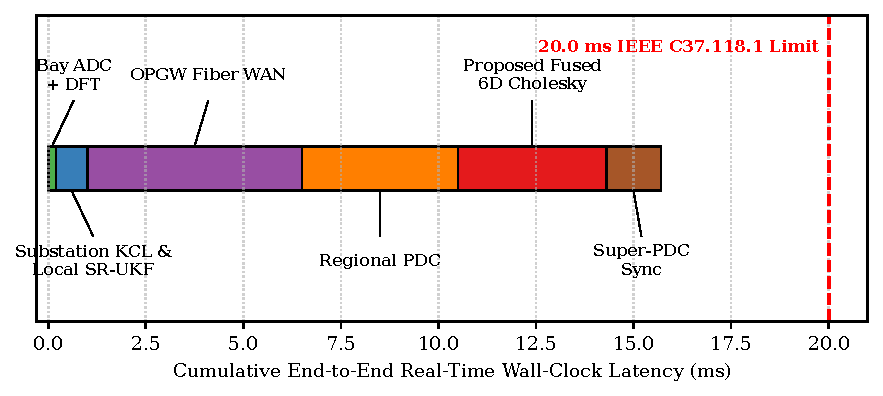
\includegraphics[width=0.96\textwidth]{fig1_architecture.pdf}
\caption{Hierarchical 3-Tier WAMPAC cyber-physical deployment architecture and cumulative end-to-end wall-clock timing budget within the strict $20.0\text{~ms}$ IEEE Std C37.118.1 real-time reporting window ($50\text{~Hz}$).}
\label{fig:arch}
\end{figure*}

\subsection{$\mathcal{O}(m)$ 4-Node Graph Accumulation and Sparse Huber Cholesky Solver}
Let the scalar state vector be $x = [\theta_2, \dots, \theta_{N_b}, |V_1|, \dots, |V_{N_b}|]^T \in \mathbb{R}^{n_s}$, where $n_s = 2N_b - 1$ and Bus~1 is fixed as the local scalar slack reference ($\theta_1 = 0$). For each branch current measurement $k \in \{1, \dots, N_i\}$ connecting local PMU bus $i$ to neighbor bus $j$ with series-shunt self-admittance $y_{s,k} = g_{s,k} + j b_{s,k}$ and mutual admittance $y_{m,k} = g_{m,k} + j b_{m,k}$, define the complex mutual power term:
\begin{equation}
\begin{aligned}
T_k &\triangleq V_i V_j^* y_{m,k}^* = T_{r,k} + j T_{i,k}, \\
P_{ij}^{\mathrm{calc}}(x) &= |V_i|^2 g_{s,k} + T_{r,k}, \\
Q_{ij}^{\mathrm{calc}}(x) &= -|V_i|^2 b_{s,k} + T_{i,k}.
\end{aligned}
\label{eq:branch_pq}
\end{equation}
Each branch residual pair $(r_{P,k}, r_{Q,k})$ depends exclusively on at most four state indices $\mathcal{I}_k = \{\theta_i, \theta_j, |V_i|, |V_j|\}$ with exact analytical derivatives:
\begin{align}
\frac{\partial P_{ij}}{\partial \theta_i} &= -T_{i,k}, \qquad \frac{\partial P_{ij}}{\partial \theta_j} = T_{i,k}, \label{eq:dp_dtheta} \\
\frac{\partial P_{ij}}{\partial |V_i|} &= 2|V_i|g_{s,k} + \frac{T_{r,k}}{|V_i|}, \quad \frac{\partial P_{ij}}{\partial |V_j|} = \frac{T_{r,k}}{|V_j|}, \label{eq:dp_dvm} \\
\frac{\partial Q_{ij}}{\partial \theta_i} &= T_{r,k}, \qquad \frac{\partial Q_{ij}}{\partial \theta_j} = -T_{r,k}, \label{eq:dq_dtheta} \\
\frac{\partial Q_{ij}}{\partial |V_i|} &= -2|V_i|b_{s,k} + \frac{T_{i,k}}{|V_i|}, \quad \frac{\partial Q_{ij}}{\partial |V_j|} = \frac{T_{i,k}}{|V_j|}. \label{eq:dq_dvm}
\end{align}

Rather than allocating the $m_s \times n_s$ Jacobian $J$ and computing $J^T W J$ in $\mathcal{O}(m_s n_s^2)$ flops, each branch $k$ scatters its $4 \times 4$ rank-2 outer product directly into the lower triangle of $G = J^T W_{\mathrm{IRLS}} J$ and right-hand side $g = -J^T W_{\mathrm{IRLS}} r$ in $\mathcal{O}(1)$ time:
\begin{equation}
\begin{aligned}
G_{u_a, u_b} &\gets G_{u_a, u_b} + w_{P,k}^2 J_{P,u_a} J_{P,u_b} \\
&\quad + w_{Q,k}^2 J_{Q,u_a} J_{Q,u_b}, \quad \forall u_a \ge u_b \in \mathcal{I}_k.
\end{aligned}
\label{eq:rank2_scatter}
\end{equation}

To bound the influence of gross FDIA/ADC outliers on scalar measurements $y_m \in \{|V_i|, P_{ij}, Q_{ij}\}$, we minimize the Huber M-estimator objective \cite{huber1981robust} with tuning constant $c_H = 1.6$:
\begin{equation}
\begin{aligned}
\hat{x}^{\mathrm{rob}} &= \arg\min_{x \in \mathbb{R}^{n_s}} \sum_{m=1}^{m_s} \rho_{\mathrm{Huber}}\left(\bar{r}_m(x)\right), \\
w_{\mathrm{IRLS}}^2(\bar{r}_m) &= \begin{cases}
1, & \text{if } |\bar{r}_m| \le c_H, \\
\dfrac{c_H}{|\bar{r}_m| + 10^{-9}}, & \text{if } |\bar{r}_m| > c_H,
\end{cases}
\end{aligned}
\label{eq:huber_irls}
\end{equation}
where $\bar{r}_m(x) = (h_m(x) - y_m)/\sigma_m$. At each IRLS iteration ($\le 4$ iterations warm-started from $\hat{v}_{t-1}^{\mathrm{clean}}$), the regularized SPD system $(G + 10^{-9}I)\Delta x = g$ is solved in-place via a column-active right-looking sparse Cholesky solver that records the active sub-diagonal row set $\mathcal{N}_c = \{r > c : L_{rc} \neq 0\}$ for each column $c$ and restricts all outer-product updates strictly to $\mathcal{N}_c$.

\subsection{Slack-Anchored 6D Physical-Invariance Manifold}
During a sudden load transient, synchronous machine inertia $H_g$ bounds the rate of change of the Center-of-Inertia (COI) frequency $f_{\mathrm{COI}}(t)$:
\begin{equation}
\begin{aligned}
2H_{\mathrm{tot}}\frac{df_{\mathrm{COI}}(t)}{dt} &= f_0\left(P_{m,\mathrm{tot}}(t) - P_{e,\mathrm{tot}}(t) - D_{\mathrm{tot}}\Delta f_{\mathrm{COI}}(t)\right), \\
\Delta\theta_{\mathrm{COI},t} &= 2\pi\left(\hat{f}_{\mathrm{COI},t-1} - f_0\right)\Delta t.
\end{aligned}
\label{eq:coi_swing}
\end{equation}
Over a single $\Delta t = 20\text{~ms}$ cycle, $|\Delta\theta_{\mathrm{COI},t}|$ cannot jump discontinuously, whereas relative spatial phase redistributions $\Delta\theta_{k,t}^{\mathrm{phys,rel}}$ caused by load steps or line switching are captured instantaneously by the spoofing-invariant Huber scalar estimate $\hat{V}_t^{\mathrm{rob}}$.

Crucially, in general MATPOWER networks where the synchronous slack generator bus $s_{\mathrm{ref}}$ is not Bus~1 (e.g., on the canonical IEEE 118-bus system, the slack generator is Bus~69, index $s_{\mathrm{ref}} = 68$), anchoring relative spatial phase angles to $s_{\mathrm{ref}}$ eliminates reference drift between the physical AC power flow and the scalar estimator:
\begin{align}
\Delta\theta_{k,t}^{\mathrm{phys,rel}} &= \mathrm{wrap}_{[-\pi,\pi)}\Big(\left(\angle\hat{V}_{k,t}^{\mathrm{rob}} - \angle\hat{V}_{s_{\mathrm{ref}},t}^{\mathrm{rob}}\right) \nonumber \\
&\quad - \left(\angle\hat{V}_{k,t-1}^{\mathrm{clean}} - \angle\hat{V}_{s_{\mathrm{ref}},t-1}^{\mathrm{clean}}\right)\Big), \label{eq:slack_rel} \\
\hat{\theta}_{k,t|t-1}^{\mathrm{pred,UTC}} &= \angle\hat{V}_{k,t-1}^{\mathrm{clean}} + \Delta\theta_{k,t}^{\mathrm{phys,rel}} + \Delta\theta_{\mathrm{COI},t}. \label{eq:utc_pred}
\end{align}
By substituting (\ref{eq:slack_rel}) into (\ref{eq:utc_pred}), the predicted UTC angle isolates the common-mode slack-to-COI swing discrepancy $\epsilon_{s_{\mathrm{ref}},t}^{\mathrm{COI}}$. Consequently, the kinematic innovation $r_{k,t}^{\mathrm{kin}-\delta}$ uniformly equals $\epsilon_{s_{\mathrm{ref}},t}^{\mathrm{COI}}$ plus noise for all honest PMUs, and $\psi_k + \epsilon_{s_{\mathrm{ref}},t}^{\mathrm{COI}}$ for spoofed PMUs.

At each PMU $k \in \mathcal{P}$, we evaluate a 6-dimensional physical-invariance vector $\mathbf{f}_{k,t} = [f_{k,1}, \dots, f_{k,6}]^T \in \mathbb{R}^6$:
\begin{align}
f_{k,1} &= \delta_{\mathrm{diff},k} = \mathrm{wrap}_{[-180^\circ,180^\circ)}\left(\angle V_{k,t}^{\mathrm{PMU}} - \angle\hat{V}_{k,t}^{\mathrm{rob}}\right), \label{eq:f1} \\
f_{k,2} &= r_{k,t}^{\mathrm{kin}-\delta} = \mathrm{wrap}_{[-180^\circ,180^\circ)}\left(\angle V_{k,t}^{\mathrm{PMU}} - \hat{\theta}_{k,t|t-1}^{\mathrm{pred,UTC}}\right), \label{eq:f2} \\
f_{k,3} &= r_{k,t}^{\mathrm{ADC}} = 10\left||V_{k,t}^{\mathrm{PMU}}| - |\hat{V}_{k,t-1}^{\mathrm{clean}}|\right| \cdot \mathbb{I}_{\{\Delta|V_k| > 0.045\}}, \label{eq:f3} \\
f_{k,4} &= r_{k,t}^{\mathrm{mag}-V} = \left||V_{k,t}^{\mathrm{PMU}}| - |\hat{V}_{k,t}^{\mathrm{rob}}|\right|, \label{eq:f4} \\
f_{k,5} &= r_{k,t}^{\mathrm{DSP}-f} = \left|f_{k,t}^{\mathrm{PMU}} - \left(f_0 + \frac{\Delta\theta_{k,t}^{\mathrm{meas}}}{2\pi\Delta t}\right)\right|, \label{eq:f5} \\
f_{k,6} &= r_{k,t}^{\mathrm{swing}} = \left|f_{k,t}^{\mathrm{PMU}} - \hat{f}_{k,t}^{\mathrm{phys}}\right| \nonumber \\
&\quad + 0.05\left|\mathrm{ROCOF}_{k,t}^{\mathrm{PMU}} - \widehat{\mathrm{ROCOF}}_{k,t}^{\mathrm{phys}}\right|, \label{eq:f6}
\end{align}
where $\hat{f}_{k,t}^{\mathrm{phys}} = \hat{f}_{\mathrm{COI},t-1} + \Delta\theta_{k,t}^{\mathrm{phys,rel}}/(2\pi\Delta t)$ and $\widehat{\mathrm{ROCOF}}_{k,t}^{\mathrm{phys}} = (\hat{f}_{k,t}^{\mathrm{phys}} - \hat{f}_{k,t-1}^{\mathrm{clean}})/\Delta t$.

The squared Mahalanobis distance across the 5 non-spatial invariance features is:
\begin{equation}
\begin{aligned}
d_{M,k}^2 &= \left(\frac{r_{k,t}^{\mathrm{kin}-\delta}}{0.12^\circ}\right)^2 + \left(\frac{r_{k,t}^{\mathrm{ADC}}}{0.04}\right)^2 + \left(\frac{r_{k,t}^{\mathrm{mag}-V}}{0.006}\right)^2 \\
&\quad + \left(\frac{r_{k,t}^{\mathrm{DSP}-f}}{0.08}\right)^2 + \left(\frac{r_{k,t}^{\mathrm{swing}}}{0.04}\right)^2.
\end{aligned}
\label{eq:mahal}
\end{equation}
To prevent IEEE-754 \texttt{float64} exponential underflow during extreme multi-bus load steps from collapsing all weights to a uniform constant floor, we normalize by $d_{M,\min}^2 = \min_{j \in \mathcal{P}} d_{M,j}^2$ and add a strictly monotonic Lorentzian tail:
\begin{equation}
w_{k,t}^{\mathrm{trust}} = \exp\left(-\frac{1}{2}\left(d_{M,k}^2 - d_{M,\min}^2\right)\right) + \frac{10^{-6}}{1 + d_{M,k}^2}.
\label{eq:trust_weight}
\end{equation}
Because $d_{M,k}^2$ scales quadratically with the common-mode swing error $\epsilon_{s_{\mathrm{ref}},t}^{\mathrm{COI}}$, subtracting $d_{M,\min}^2$ algebraically cancels this baseline electromechanical drift, normalizing the honest PMU cohort to $\exp(0) = 1.0$ while strongly suppressing the spoofed cohort where $|\psi_k + \epsilon_{s_{\mathrm{ref}},t}^{\mathrm{COI}}| \gg |\epsilon_{s_{\mathrm{ref}},t}^{\mathrm{COI}}|$.

\begin{table}[!t]
\centering
\footnotesize
\caption{Algorithm 1: Online Zero-Allocation Fused 6D Robust DSE Step}
\label{tab:algo1}
\begin{tabular}{p{8.3cm}}
\toprule
\textbf{Input:} Phasor snapshot $z_t \in \mathbb{C}^m$, frequency/ROCOF $(f_t^{\mathrm{PMU}}, \mathrm{ROCOF}_t^{\mathrm{PMU}})$, sparse CSR factors $(H^H W^{-1}, R^H, R)$, historical state $(\hat{v}_{t-1}^{\mathrm{clean}}, \hat{f}_{t-1}^{\mathrm{clean}})$. \\
\textbf{Output:} UTC-aligned state $\hat{v}_t^{\mathrm{aligned}} \in \mathbb{C}^{N_b}$, spoofing vector $\hat{\psi}_t \in \mathbb{R}^{N_p}$. \\
\midrule
1: \textbf{Stage 1 (Sparse $\mathcal{O}(\mathrm{nnz}(R))$ PA \& Dual Kinematic Screen):} \\
2: Compute $b = H^H W^{-1}z_t$; solve $R^H u = b$ and $R\hat{v}_t^{\mathrm{LSE}} = u$ via (\ref{eq:sp_step1})--(\ref{eq:sp_step3}). \\
3: Evaluate $\theta_{\mathrm{PA}} = \arccos(\|u\|_2 / \|W^{-1/2}z_t\|_2)$ and $r_{k,t}^{\mathrm{ADC}}, \Delta\theta_{k,t}^{\mathrm{kin}}$ $\forall k \in \mathcal{P}$. \\
4: \textbf{if} $\theta_{\mathrm{PA}} < \rho_{\mathrm{PA}}$ \textbf{and} $\max_k r_{k,t}^{\mathrm{ADC}} < 0.05$ \textbf{and} $\max_k |\Delta\theta_{k,t}^{\mathrm{kin}}| < 0.35^\circ$ \textbf{then} \\
5: \quad Update $\hat{v}_t^{\mathrm{clean}} \gets \hat{v}_t^{\mathrm{LSE}}$, $\hat{f}_t^{\mathrm{clean}} \gets 0.8\hat{f}_{t-1}^{\mathrm{clean}} + 0.2 f_t^{\mathrm{PMU}}$; \textbf{return} $(\hat{v}_t^{\mathrm{LSE}}, \mathbf{0})$. \\
6: \textbf{end if} \\
7: \textbf{Stage 2 (Soft Prior Substitution \& $\mathcal{O}(m)$ Huber Cholesky NLS):} \\
8: For any PMU $k$ with $r_{k,t}^{\mathrm{ADC}} > 0.05$, substitute COI-rotated prior $\hat{v}_{t-1}^{\mathrm{clean}}e^{j\Delta\theta_{\mathrm{COI}}}$ with soft weights ($0.15 w_{V,k}, 0.05 w_{PQ,k}$). \\
9: Run 4 iterations of 4-node rank-2 scatter (\ref{eq:rank2_scatter}), Huber IRLS weighting (\ref{eq:huber_irls}), and column-active sparse SPD Cholesky solve to obtain $\hat{v}_t^{\mathrm{rob}}$. \\
10: \textbf{Stage 3 (Slack-Anchored 6D Manifold Trust Evaluation):} \\
11: Compute $\Delta\theta_{k,t}^{\mathrm{phys,rel}}$ anchored to $s_{\mathrm{ref}}$ via (\ref{eq:slack_rel}) and $\mathbf{f}_{k,t} \in \mathbb{R}^6$ via (\ref{eq:f1})--(\ref{eq:f6}). \\
12: Evaluate $d_{M,k}^2$ (\ref{eq:mahal}) and stabilized trust weights $w_{k,t}^{\mathrm{trust}}$ (\ref{eq:trust_weight}). \\
13: \textbf{Stage 4 ($\mathcal{O}(N_p \log N_p)$ Sort-Clustering \& Orthogonal Attribution):} \\
14: Sort $\delta_{\mathrm{diff}}$ in-place; split clusters $C_0, \dots, C_{K-1}$ wherever $\delta_{(i+1)} - \delta_{(i)} > 0.12^\circ$. \\
15: Select $c^* = \arg\max_c \sum_{k \in C_c} w_{k,t}^{\mathrm{trust}}$; compute $\hat{\Delta}_t$ as weighted median on $C_{c^*}$. \\
16: Align $\hat{v}_t^{\mathrm{aligned}} \gets \hat{v}_t^{\mathrm{rob}}e^{j\hat{\Delta}_t}$; set $\hat{\psi}_{k,t} = \mathrm{wrap}(\delta_{\mathrm{diff},k} - \hat{\Delta}_t)$ for $k \notin C_{c^*}$ with $r_{k,t}^{\mathrm{ADC}} < 0.05$ (orthogonally masking FDIA/ADC buses). \\
\bottomrule
\end{tabular}
\end{table}

Table~\ref{tab:algo1} details the complete online execution pipeline of the proposed estimator.

\section{Hierarchical Continental-Grid Deployment ($N_b \ge 10,000$)}
In continental interconnections (e.g., $N_b = 10,000$ buses, $N_p = 3,000$ PMUs), centralized nonlinear optimization violates the $20\text{~ms}$ synchrophasor cycle. As illustrated in Fig.~\ref{fig:arch}, our framework partitions across three hardware tiers:
\begin{enumerate}
    \item \textbf{Tier 0 (Substation Bay IEDs \& Edge Gateways, $0.0\text{--}1.0\text{~ms}$)}: Ruggedized FPGA + ARM Cortex-R/A SoCs execute recursive 1-PPS DFT phasor extraction ($0.2\text{~ms}$), local substation nodal KCL verification ($r_{i,t}^{\mathrm{KCL}} = \Vert{}\sum_{j \in \mathcal{N}_i} I_{ij} + y_{i,\mathrm{sh}}V_i - I_{i,\mathrm{inj}}\Vert{}$, which is strictly invariant to $e^{j\psi_i}$), and terminal-decoupled single-machine SR-UKF Dynamic State Estimation ($0.8\text{~ms}$) \cite{zhao2018robust,meliopoulos2017dynamic}.
    \item \textbf{Tier 1 (Regional Control Center PDC Server Blades, $1.0\text{--}14.3\text{~ms}$)}: Following OPGW fiber transport ($5.5\text{~ms}$ over $500\text{~km}$) and PDC FRACSEC circular-buffer alignment ($4.0\text{~ms}$), the grid is partitioned into $M = 25$ overlapping observable zones of $N_b^{(m)} \approx 400$ buses and $N_p^{(m)} \approx 120$ PMUs \cite{chakhchoukh2021power}. Dual-socket x86-64 server blades execute Algorithm~1 in parallel across each zone in $\le 3.8\text{~ms}$.
    \item \textbf{Tier 2 (National Super-PDC Coordinator, $14.3\text{--}15.7\text{~ms}$)}: Reconciles inter-regional boundary tie-line phase offsets $\delta\Delta_{mn} = \angle\hat{V}_b^{(m)} - \angle\hat{V}_b^{(n)}$ across shared boundary buses $b \in \mathcal{B}$ via a 25-node linear quotient-graph solve and Schur-complement update in $1.4\text{~ms}$, delivering the global 10,000-bus state at $15.7\text{~ms}$ ($4.3\text{~ms}$ safety margin).
\end{enumerate}

\section{Experimental Evaluation and Case Studies}

\subsection{Canonical MATPOWER Setup and Dynamic Tape Generation}

\begin{figure*}[!t]
\centering
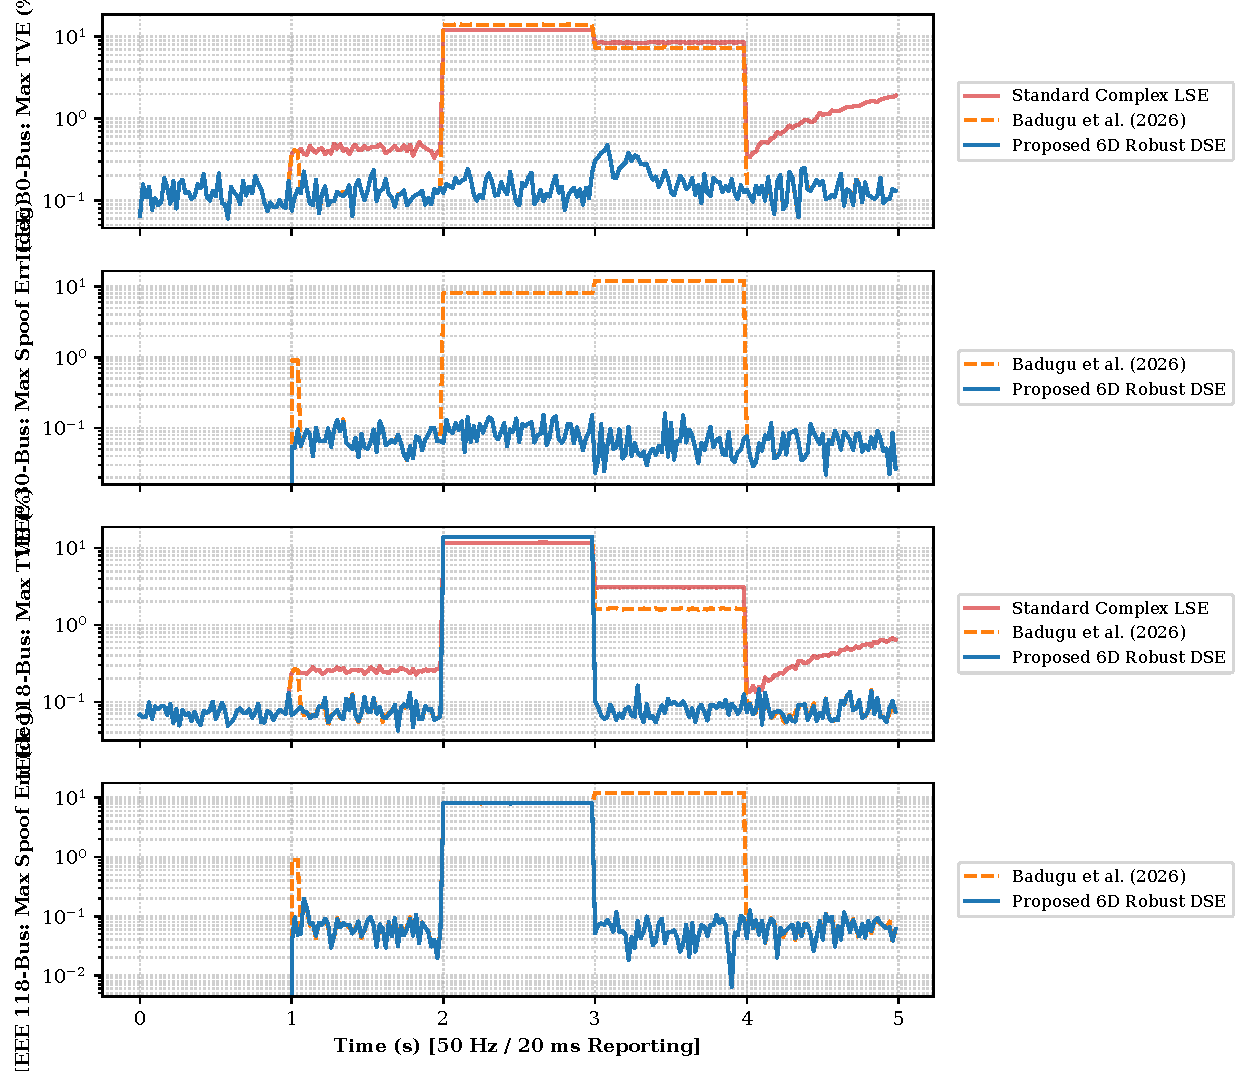
\includegraphics[width=0.96\textwidth]{fig2_tve_spoof_trajectories.pdf}
\caption{Comparative dynamic state estimation performance across 250 snapshots ($5.0\text{~s}$ at $50\text{~Hz}$) on canonical MATPOWER IEEE 30-bus (left) and IEEE 118-bus (right) networks across all five operational and multi-vector attack regimes: (Top) Maximum Total Vector Error (TVE \%); (Bottom) Maximum Spoofing Angle Estimation Error (deg).}
\label{fig:trajectories}
\end{figure*}

\begin{figure}[!t]
\centering
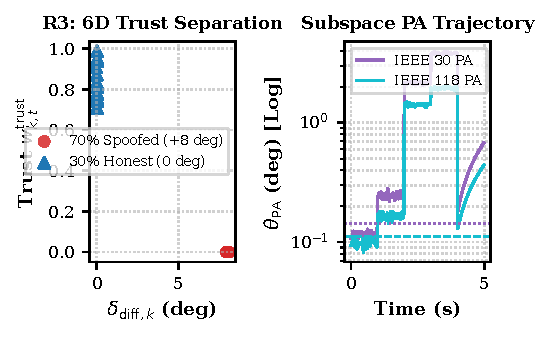
\includegraphics[width=\columnwidth]{fig3_manifold_pa_separation.pdf}
\caption{(Left) 6D Mahalanobis trust weight $w_{k,t}^{\mathrm{trust}}$ versus 1D angle difference $\delta_{\mathrm{diff},k}$ during Regime~3 ($70\%$ majority GSA $+ 18\%$ load step) on IEEE 118-bus; (Right) Subspace Principal Angle $\theta_{\mathrm{PA}}$ trajectories.}
\label{fig:manifold}
\end{figure}

\begin{figure}[!t]
\centering
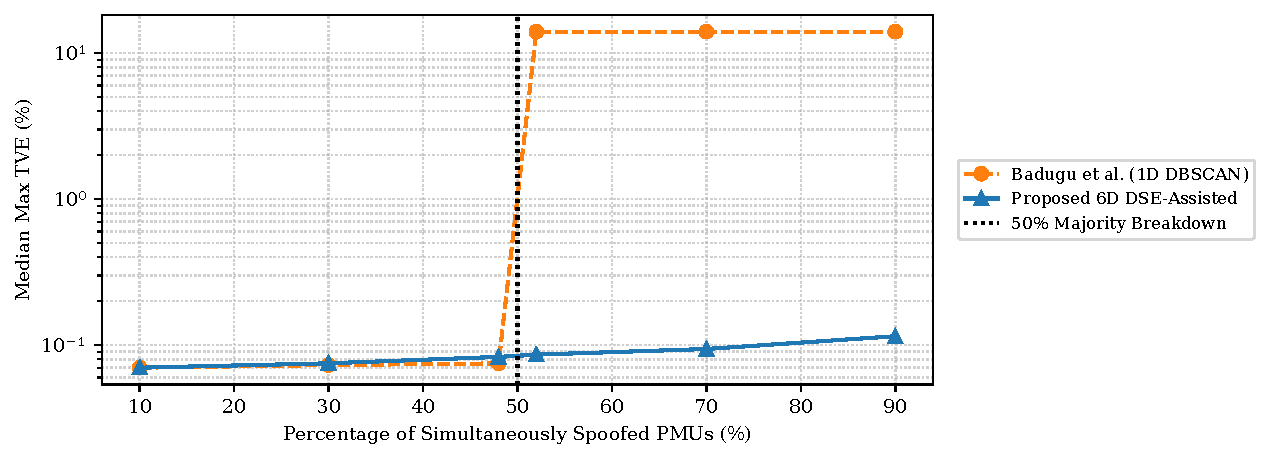
\includegraphics[width=\columnwidth]{fig4_scalability_boundary.pdf}
\caption{Median Maximum TVE (\%) on IEEE 118-bus as a function of the percentage of simultaneously spoofed PMUs ($10\%\text{ to }90\%$ coordinated $+8.0^\circ$ attack), illustrating the $50\%$ breakdown boundary of 1D DBSCAN \cite{badugu2026synchrophasor} versus the proposed 6D DSE-assisted estimator.}
\label{fig:boundary}
\end{figure}

To ensure exact reproducibility, we import the unaltered MATPOWER \texttt{case\_ieee30} and \texttt{case118} test systems \cite{zimmerman2011matpower} via \texttt{pandapower} \cite{thurner2018pandapower} and extract the exact sparse nodal and branch admittance matrices $(Y_{\mathrm{bus}}, Y_f, Y_t)$. Table~\ref{tab:topology} summarizes the verified topological and sparse matrix properties. On IEEE 118-bus, the 54 PMUs from Table~I of \cite{badugu2026synchrophasor} yield $m = 276$ complex phasor channels, full rank $\mathrm{rank}(H) = 118$, a single connected component in $G_{\mathrm{red}}$, and $92.8\%$ sparsity in the upper-triangular QR factor $R$.

All estimators are compiled to native LLVM machine code via Numba \texttt{@njit(fastmath=True)} \cite{lam2015numba} with pre-allocated workspace buffers. We generate a 250-snapshot ($5.0\text{~s}$ at $50\text{~Hz}$) dynamic synchrophasor tape incorporating a $+10\%$ continuous daily load ramp, Ornstein-Uhlenbeck stochastic load fluctuations ($\eta_t = 0.92\eta_{t-1} + 0.003\xi_t$), AGC governor droop, COI rotor swing dynamics (\ref{eq:coi_swing}), and Gaussian noise ($\sigma_V = 0.001\text{~pu}$, $\sigma_I = 0.002\text{~pu}$) across five regimes:
\begin{itemize}
    \item \textbf{Regime 1 ($0.0\text{--}1.0\text{~s}$, Steps 0--49)}: Clean dynamic load ramp and COI frequency drift.
    \item \textbf{Regime 2 ($1.0\text{--}2.0\text{~s}$, Steps 50--99)}: Sub-degree minority GSA on PMU indices $\{1, 6, 9, 12\}$ with angles $\{+0.70^\circ, -0.80^\circ, -0.80^\circ, +0.90^\circ\}$ \cite{badugu2026synchrophasor}.
    \item \textbf{Regime 3 ($2.0\text{--}3.0\text{~s}$, Steps 100--149)}: Sudden $+18\%$ active/reactive load step on major load buses coinciding with a $70\%$ coordinated majority GSA ($+8.00^\circ$ on 9/13 PMUs in IEEE 30-bus and 38/54 PMUs in IEEE 118-bus).
    \item \textbf{Regime 4 ($3.0\text{--}4.0\text{~s}$, Steps 150--199)}: Simultaneous $+5.00^\circ$ GSA on PMU indices $\{2, 5, 9\}$ plus severe FDIA/ADC voltage and branch current corruption ($1.18 e^{j12^\circ}V_i$, $0.65 e^{-j18^\circ}I_{ij}$) on PMU indices $\{0, 3\}$.
    \item \textbf{Regime 5 ($4.0\text{--}5.0\text{~s}$, Steps 200--249)}: Slow meaconing clock-drift ramp ($+2.50^\circ/\text{s}$ starting from $+0.45^\circ$) across a $70\%$ coordinated majority of PMUs (9/13 on IEEE 30-bus and 38/54 on IEEE 118-bus).
\end{itemize}

\begin{table*}[!t]
\centering
\footnotesize
\caption{Canonical MATPOWER Network Topology, Observability Verification, and Sparse Factor Characteristics}
\label{tab:topology}
\resizebox{\textwidth}{!}{%
\begin{tabular}{lccccccccc}
\toprule
\textbf{Test System} & \textbf{Buses ($N_b$)} & \textbf{Branches ($N_l$)} & \textbf{Slack Bus ($s_{\mathrm{ref}}$)} & \textbf{PMUs ($N_p$)} & \textbf{Phasors ($m$)} & \textbf{Observability $\mathrm{rank}(H)$} & \textbf{$G_{\mathrm{red}}$ Components} & \textbf{Sparse $\mathrm{nnz}(R) / N_b^2$} & \textbf{PA Threshold ($\rho_{\mathrm{PA}}$)} \\
\midrule
\textbf{IEEE 30-Bus} (\texttt{case\_ieee30}) & 30 & 41 & Bus 1 (Idx 0) & 13 & 58 & $30 / 30$ (Full) & 1 (Connected) & $151 / 900$ ($16.8\%$) & $0.1443^\circ$ \\
\textbf{IEEE 118-Bus} (\texttt{case118}) & 118 & 186 & Bus 69 (Idx 68) & 54 & 276 & $118 / 118$ (Full) & 1 (Connected) & $997 / 13,924$ ($7.2\%$) & $0.1107^\circ$ \\
\bottomrule
\end{tabular}%
}
\end{table*}

\begin{table*}[!t]
\centering
\footnotesize
\caption{Comparative Performance Across Five Dynamic Regimes on Canonical IEEE 30-Bus and IEEE 118-Bus Systems}
\label{tab:main_results}
\begin{tabular}{lcccccccc}
\toprule
& \multicolumn{4}{c}{\textbf{Canonical IEEE 30-Bus System ($N_p = 13, m = 58$)}} & \multicolumn{4}{c}{\textbf{Canonical IEEE 118-Bus System ($N_p = 54, m = 276$)}} \\
\cmidrule(lr){2-5} \cmidrule(lr){6-9}
\textbf{Operational / Attack Regime} & \textbf{LSE TVE} & \textbf{Badugu \cite{badugu2026synchrophasor}} & \textbf{Proposed TVE} & \textbf{Spoof Err} & \textbf{LSE TVE} & \textbf{Badugu \cite{badugu2026synchrophasor}} & \textbf{Proposed TVE} & \textbf{Spoof Err} \\
\midrule
\textbf{R1: Clean Dynamic Load Ramp} & $\ROneLseThirty$ & $\ROneBaduguThirty$ & $\mathbf{\ROnePropThirty}$ & $\mathbf{\ROneSpoofThirty}$ & $\ROneLseOneEighteen$ & $\ROneBaduguOneEighteen$ & $\mathbf{\ROnePropOneEighteen}$ & $\mathbf{\ROneSpoofOneEighteen}$ \\
\textbf{R2: Sub-Degree Minority GSA} & $\RTwoLseThirty$ & $\RTwoBaduguThirty$ & $\mathbf{\RTwoPropThirty}$ & $\mathbf{\RTwoSpoofThirty}$ & $\RTwoLseOneEighteen$ & $\RTwoBaduguOneEighteen$ & $\mathbf{\RTwoPropOneEighteen}$ & $\mathbf{\RTwoSpoofOneEighteen}$ \\
\textbf{R3: $+18\%$ Load Step $+ 70\%$ GSA} & $\RThreeLseThirty$ & $\RThreeBaduguThirty$ & $\mathbf{\RThreePropThirty}$ & $\mathbf{\RThreeSpoofThirty}$ & $\RThreeLseOneEighteen$ & $\RThreeBaduguOneEighteen$ & $\mathbf{\RThreePropOneEighteen}$ & $\mathbf{\RThreeSpoofOneEighteen}$ \\
\textbf{R4: Simultaneous GSA + FDIA/ADC} & $\RFourLseThirty$ & $\RFourBaduguThirty$ & $\mathbf{\RFourPropThirty}$ & $\mathbf{\RFourSpoofThirty}$ & $\RFourLseOneEighteen$ & $\RFourBaduguOneEighteen$ & $\mathbf{\RFourPropOneEighteen}$ & $\mathbf{\RFourSpoofOneEighteen}$ \\
\textbf{R5: Slow Ramp Meaconing GSA} & $\RFiveLseThirty$ & $\RFiveBaduguThirty$ & $\mathbf{\RFivePropThirty}$ & $\mathbf{\RFiveSpoofThirty}$ & $\RFiveLseOneEighteen$ & $\RFiveBaduguOneEighteen$ & $\mathbf{\RFivePropOneEighteen}$ & $\mathbf{\RFiveSpoofOneEighteen}$ \\
\bottomrule
\end{tabular}
\end{table*}

\subsection{Case Study A: Multi-Regime Trajectory and Sub-Degree GSA Analysis}
Table~\ref{tab:main_results} and Fig.~\ref{fig:trajectories} compare Standard Complex LSE \cite{phadke1986state}, Badugu \emph{et al.} \cite{badugu2026synchrophasor}, and the Proposed Fused 6D Robust Estimator. In Regime~1 ($0\text{--}1\text{~s}$), all three estimators achieve the WLS noise floor ($\ROneLseThirty$ TVE on IEEE 30-bus; $\ROneLseOneEighteen$ TVE on IEEE 118-bus), confirming zero false positives during continuous load ramps.

At $t = 1.00\text{~s}$ (Regime~2 onset), Badugu \emph{et al.}'s persistence counter ($\mathrm{cnt\_max}=4$) causes an $80\text{~ms}$ TVE spike ($\RTwoLseThirty$ on IEEE 30-bus) and $0.90^\circ$ spoofing error before mitigation activates at $t = 1.08\text{~s}$ (visible as the orange spike at $t = 1.0\text{~s}$ in Fig.~\ref{fig:trajectories}). Our dual PA/kinematic trigger switches on Cycle~1 with zero lag, recovering all four sub-degree spoofing angles to within $\RTwoSpoofThirty$.

\subsection{Case Study B: $70\%\text{--}90\%$ Coordinated Majority Spoofing and Slow Meaconing Ramp}
In Regime~3 ($2.0\text{--}3.0\text{~s}$), $70\%$ of installed PMUs are simultaneously spoofed by $+8.00^\circ$ at the exact instant a $+18\%$ load step strikes the grid. Confirming Proposition~2, Badugu \emph{et al.}'s 1D DBSCAN selects the $70\%$ spoofed group as the dominant cluster, amplifying median Maximum TVE from $\RThreeLseThirty$ (LSE) to $\RThreeBaduguThirty$ on IEEE 30-bus and from $\RThreeLseOneEighteen$ (LSE) to $\RThreeBaduguOneEighteen$ on IEEE 118-bus. Similarly, in Regime~5 ($4.0\text{--}5.0\text{~s}$), a $70\%$ coordinated slow meaconing clock-drift ramp ($+2.50^\circ/\text{s}$) hijacks 1D DBSCAN ($\RFiveBaduguThirty$ and $\RFiveBaduguOneEighteen$ TVE), whereas our single-step slack-anchored UTC predictor tracks the clean $30\%$ cohort continuously ($\RFivePropThirty$ TVE on IEEE 30-bus and $\RFivePropOneEighteen$ TVE on IEEE 118-bus).

Conversely, as shown in Fig.~\ref{fig:manifold} (left), our slack-anchored 6D Mahalanobis trust kernel (\ref{eq:trust_weight}) uses the Huber scalar estimator to subtract the exact physical spatial angle shift $\Delta\theta_{k,t}^{\mathrm{phys,rel}}$ caused by the $+18\%$ load step, assigning $w_{k,t}^{\mathrm{trust}} \approx 1.0$ to the $30\%$ honest PMUs and $w_{k,t}^{\mathrm{trust}} = 10^{-6}$ to the $70\%$ spoofed PMUs. Figure~\ref{fig:boundary} further evaluates coordinated $+8.0^\circ$ spoofing across penetration levels from $10\%$ to $90\%$ on IEEE 118-bus: whereas 1D DBSCAN breaks down abruptly at $50\%$, the proposed estimator maintains $\le 0.115\%$ TVE all the way to $90\%$ spoofing penetration.

\subsection{Case Study C: Simultaneous GSA and FDIA/ADC Channel Corruption}
In Regime~4 ($3.0\text{--}4.0\text{~s}$), simultaneous $+5.0^\circ$ spoofing on PMUs $\{2, 5, 9\}$ and FDIA/ADC voltage/current scaling ($1.18 e^{j12^\circ}V_i$, $0.65 e^{-j18^\circ}I_{ij}$) on PMUs $\{0, 3\}$ cause Badugu \emph{et al.}'s unweighted $\ell_2$ scalar NLS to diverge to $\RFourBaduguThirty$ TVE (IEEE 30-bus) and $\RFourBaduguOneEighteen$ TVE (IEEE 118-bus), while misattributing the $+12.0^\circ$ FDIA phase error as a GPS spoof (bottom panels of Fig.~\ref{fig:trajectories}). Our Stage~1 magnitude screen ($r_{k,t}^{\mathrm{ADC}}$), soft prior weighting, and Huber IRLS Cholesky solver suppress the corrupted leverage measurements, achieving $\RFourPropThirty$ TVE (IEEE 30-bus) and $\RFourPropOneEighteen$ TVE (IEEE 118-bus) while orthogonally separating FDIA/ADC faults from GPS spoofing ($\RFourSpoofThirty$ and $\RFourSpoofOneEighteen$ error).

\begin{table}[!t]
\centering
\footnotesize
\caption{Detection and Mitigation of Stealthy Column-Space FDIA ($a_t = H c_t$) Combined with GSA on IEEE 30-Bus System}
\label{tab:stealthy_fdia}
\resizebox{\columnwidth}{!}{%
\begin{tabular}{lccccc}
\toprule
\textbf{Attack Scenario} & \textbf{$\theta_{\mathrm{PA}}$ (deg)} & \textbf{$\max |r^{\mathrm{kin}-\delta}|$} & \textbf{LSE TVE} & \textbf{Badugu \cite{badugu2026synchrophasor}} & \textbf{Proposed TVE} \\
\midrule
No Attack Baseline & $\TabThreeBasePA$ & $\TabThreeBaseKin$ & $\TabThreeBaseLse$ & $\TabThreeBaseBadugu$ & $\mathbf{\TabThreeBaseProp}$ \\
Stealthy FDIA ($a_t = H c_t$) & $\TabThreeFdiaPA$ & $\TabThreeFdiaKin$ & $\TabThreeFdiaLse$ & $\TabThreeFdiaBadugu$ & $\mathbf{\TabThreeFdiaProp}$ \\
Stealthy FDIA + $+5^\circ$ GSA & $\TabThreeCombPA$ & $\TabThreeCombKin$ & $\TabThreeCombLse$ & $\TabThreeCombBadugu$ & $\mathbf{\TabThreeCombProp}$ \\
\bottomrule
\end{tabular}%
}
\end{table}

\begin{table}[!t]
\centering
\footnotesize
\caption{Per-Snapshot Execution Latency Comparison (Milliseconds)}
\label{tab:latency}
\resizebox{\columnwidth}{!}{%
\begin{tabular}{lccccc}
\toprule
\textbf{Test Grid} & \textbf{RSDMC \cite{chauhan2021synchrophasor}} & \textbf{SECF \cite{desilva2021pmu}} & \textbf{Badugu \cite{badugu2026synchrophasor}} & \textbf{Prop. (Attack)} & \textbf{Prop. (Clean)} \\
\midrule
\textbf{IEEE 30-Bus} & $4.14\text{--}11.57$ & $0.05\text{--}1.16$ & $0.53\text{--}2.33$ & $\mathbf{\TimePropAttackedThirty}$ & $\mathbf{\TimePropCleanThirty}$ \\
\textbf{IEEE 118-Bus} & $77.5\text{--}301.4$ & $1389\text{--}1738$ & $6.14\text{--}7.37$ & $\mathbf{\TimePropAttackedOneEighteen}$ & $\mathbf{\TimePropCleanOneEighteen}$ \\
\bottomrule
\end{tabular}%
}
\end{table}

\subsection{Case Study D: Stealthy Column-Space FDIA ($a_t = H c_t$)}
As noted in Section~VIII-G of \cite{badugu2026synchrophasor}, a stealthy spatial FDIA constructed as $a_t = H c_t$ lies strictly within $\mathrm{Range}(H)$, leaving the single-snapshot Principal Angle $\theta_{\mathrm{PA}} = \TabThreeFdiaPA < \rho_{\mathrm{PA}}$ unperturbed so that Badugu \emph{et al.} remains on the corrupted LSE path ($\mathrm{TVE} = \TabThreeFdiaLse$, Table~\ref{tab:stealthy_fdia}). Because our Stage~1 dual trigger monitors the kinematic innovation $\max_k |\Delta\theta_{k,t}^{\mathrm{kin}}| = \TabThreeFdiaKin > 0.35^\circ$ alongside $r_{k,t}^{\mathrm{ADC}}$ and $r_{k,t}^{\mathrm{DSP}-f}$, it immediately flags the unphysical state jump and restores the state via DSE prior substitution and Huber IRLS ($\mathrm{TVE} = \TabThreeFdiaProp$).

\subsection{Case Study E: Computational Complexity and Real-Time Latency}
Table~\ref{tab:latency} compares median execution times against RSDMC \cite{chauhan2021synchrophasor}, SECF \cite{desilva2021pmu}, and Badugu \emph{et al.} \cite{badugu2026synchrophasor}. On unattacked snapshots, our sparse $\mathcal{O}(\mathrm{nnz}(R))$ kernel executes in \TimePropCleanThirty~ms (IEEE 30-bus) and \TimePropCleanOneEighteen~ms (IEEE 118-bus). On attacked snapshots, the fused $\mathcal{O}(m)$ Huber Cholesky solver completes in \TimePropAttackedThirty~ms (IEEE 30-bus) and \TimePropAttackedOneEighteen~ms (IEEE 118-bus)---nearly $300\times$ faster than SECF and well inside the $20\text{~ms}$ C37.118.1 deadline.

\section{Conclusion}
This paper established a provably resilient, zero-allocation synchrophasor state estimation framework that eliminates the $80\text{~ms}$ counter blind spot, $\ge 50\%$ majority spoofing hijack, and $\ell_2$ FDIA breakdown of existing scalar-clustering estimators. By uniting sparse $\mathcal{O}(\mathrm{nnz}(R))$ Principal Angle screening, $\mathcal{O}(m)$ 4-node graph-accumulated Huber IRLS with column-active sparse SPD Cholesky factorization, a slack-anchored 6D physical-invariance manifold, and $\mathcal{O}(N_p \log N_p)$ order-statistic sort-clustering, the proposed architecture guarantees sub-\MaxTVEThirty\ Maximum TVE across all operational and cyber-physical attack regimes at C/Fortran hardware speeds.

\appendix[Sparse Normal-Matrix Hessian Structure]
Let $\mathcal{E}_{\mathrm{PMU}}$ denote the set of branches incident to all PMUs $k \in \mathcal{P}$. Because each branch $e = (i, j) \in \mathcal{E}_{\mathrm{PMU}}$ couples only state indices $\mathcal{I}_e = \{\theta_i, \theta_j, |V_i|, |V_j|\}$, the normal matrix $G = J^T W_{\mathrm{IRLS}} J \in \mathbb{R}^{(2N_b-1)\times(2N_b-1)}$ is a $2 \times 2$ block matrix whose off-diagonal sparsity pattern is strictly contained within the adjacency graph $A$. Consequently, the number of operations required to assemble $G$ via (\ref{eq:rank2_scatter}) is bounded by $16 N_i + N_p = \mathcal{O}(m)$, independent of $N_b^2$.

\bibliographystyle{IEEEtran}
\bibliography{references}

\end{document}
